\documentclass[../manual.tex]{subfiles}


\begin{document}
Within this section, we will provide some common usage examples of SWATHLib.

\section{Creating A Y-library for N-glycosylated peptide}
Here we have a precursor sequence with the id \textbf{test\_sequence} and the aa sequence \textbf{TTENDTFWKEF}, or in fasta format \par
\begin{verbatim}
	>test_sequence
	TTENDTFWKEF
\end{verbatim}

Upon input into the fasta content box and process, display similar to Figure \ref{fig:testsequenceylibrary} should appear.

\begin{figure}[h]
	\centering
	\begin{framed}
        \centering
        \begin{adjustbox}{width=1\textwidth}
			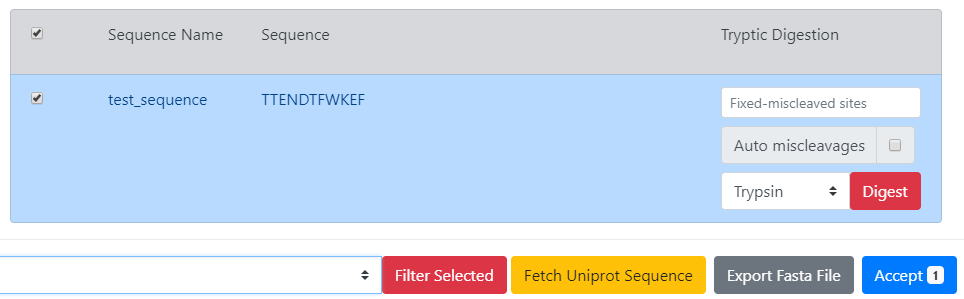
\includegraphics{test-sequence-ylibrary}
		\end{adjustbox}
		\caption{Example sequence input.}\label{fig:testsequenceylibrary}
	\end{framed}
\end{figure}


This sequence has an N-glycosylation sequon at position 4 and a tryptic digestion site right after position 9. With this library, we aimed to generate all HexNAc Y0, Y1, and Y2 transitions for the sequence at RT of 10 across all SWATH windows. The max charge allowed would be 2 and the annotated sequence at the modification position would include both RT and SWATH window value.\par


After in-silico digestion with trypsin, we would obtain two sequences (Figure \ref{fig:testsequenceylibrarydigested}), one before and one after the digestion site. The name of the sequences have also been automatically modified to show the starting and stopping positions of each digested fragment. Using the filter rule for N-glycosylation sequon, the GUI would identify and select all sequences with a sequon within those already selected.
\begin{figure}[h]
	\centering
	\begin{framed}
        \centering
        \begin{adjustbox}{width=1\textwidth}
			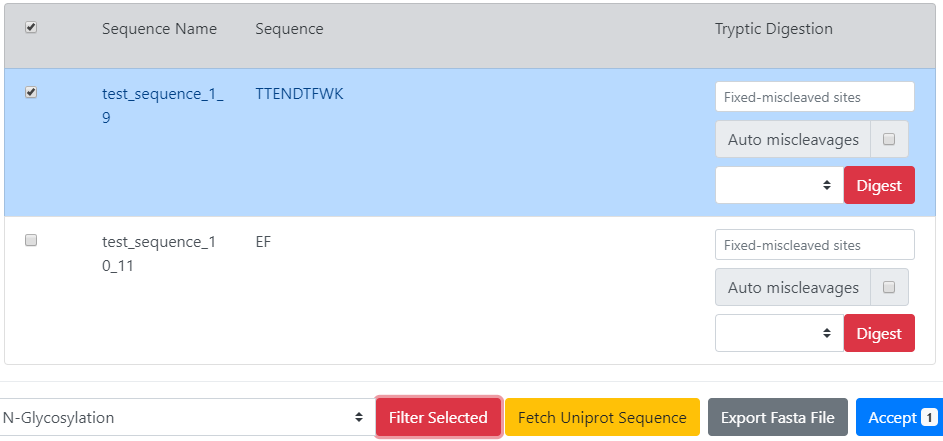
\includegraphics{test-sequence-ylibrary-digested}
		\end{adjustbox}
		\caption{Example sequence input after in-silico trypsin digestion and filtered for only those containing N-glycosylation sequon.}\label{fig:testsequenceylibrarydigested}
	\end{framed}
\end{figure}

We currently have a tryptic digested sequence containing N-glycosylation sequon but without any modification and experiment settings applied to it. These settings can be selected within the \textbf{Queryset Input Settings} panel.\par

In Figure \ref{fig:testsequenceylibrarysettings}, we have the following settings selected,
\begin{itemize}
	\item HexNAc Y0, Y1, and Y2 modifications.
	\item Retention time at 10.
	\item All SWATH windows.
	\item Y fragmentation ion-type
	\item Output sequence format include RT and SWATH window values at variable modification sites.
\end{itemize}
\begin{figure}[h]
	\centering
	\begin{framed}
        \centering
        \begin{adjustbox}{width=1\textwidth}
			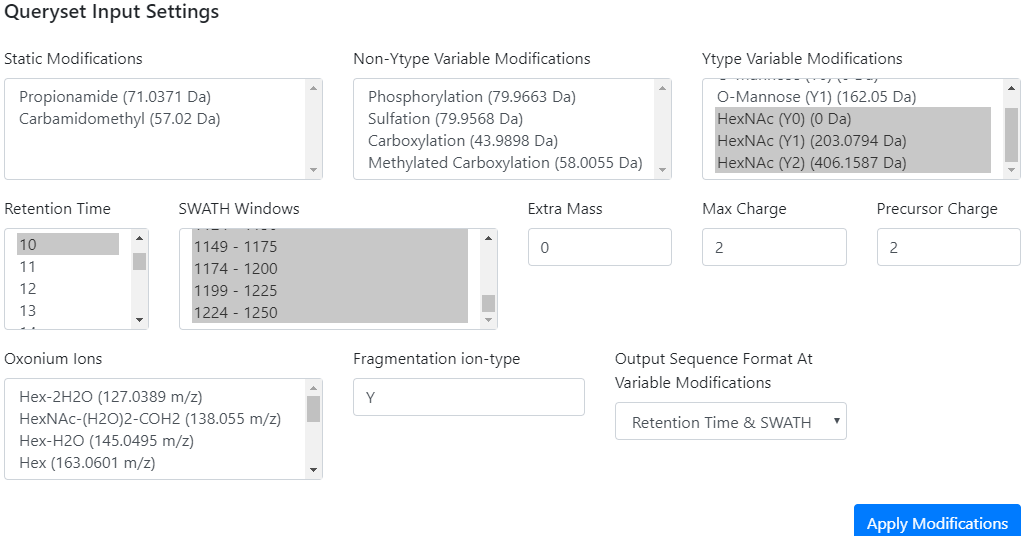
\includegraphics{test-sequence-ylibrary-settings}
		\end{adjustbox}
		\caption{Example modification settings for N-glycosylation library with 3 HexNAc Ytype transitions at RT 10 and across all default SWATH windows.}\label{fig:testsequenceylibrarysettings}
	\end{framed}
\end{figure}
After application of modification settings, the result would be display in Figure \ref{fig:testsequenceylibraryindividual}.
\begin{figure}[h]
	\centering
	\begin{framed}
        \centering
        \begin{adjustbox}{width=1\textwidth}
			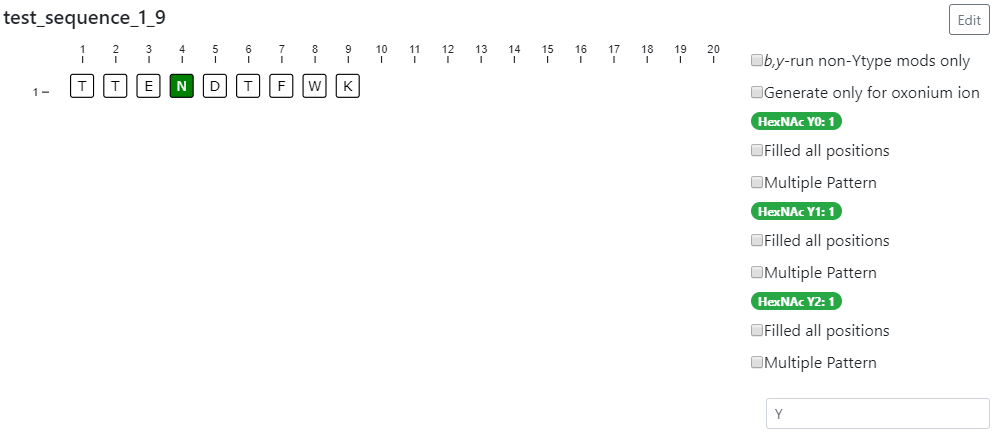
\includegraphics{test-sequence-ylibrary-individual}
		\end{adjustbox}
		\caption{Example of a sequence with the settings above applied.}\label{fig:testsequenceylibraryindividual}
	\end{framed}
\end{figure}
\end{document}